\chapter{Concrete grammar of the language} \label{anx:grammar}

\begin{figure}[!ht]

\textbf{Program:}\\
\vspace{0.2cm}
\hspace{1cm}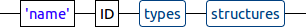
\includegraphics[scale=0.37]{./annex/images/p.png}

\textbf{types:} \hspace{6cm}\textbf{statements:}\\
\vspace{0.2cm}
\hspace{1cm}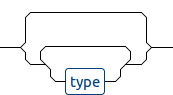
\includegraphics[scale=0.37]{./annex/images/types.png} \hspace{4cm}\hspace{1cm}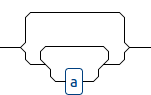
\includegraphics[scale=0.37]{./annex/images/statements.png}

\textbf{type:}\\
\vspace{0.2cm}
\hspace{1cm}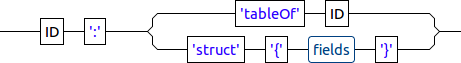
\includegraphics[scale=0.37]{./annex/images/type.png}

\textbf{fields:} \hspace{6cm} \textbf{structures:}\\
\vspace{0.2cm}
\hspace{1cm}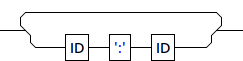
\includegraphics[scale=0.37]{./annex/images/fields.png} \hspace{4cm}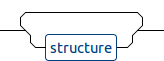
\includegraphics[scale=0.37]{./annex/images/structures.png}

\textbf{structure:}\\
\vspace{0.2cm}
\hspace{1cm}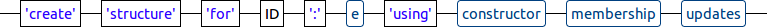
\includegraphics[scale=0.37]{./annex/images/structure.png}

\textbf{constructor:} \hspace{4.75cm} \textbf{membership:}\\
\vspace{0.2cm}
\hspace{1cm}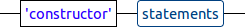
\includegraphics[scale=0.37]{./annex/images/constructor.png} \hspace{4cm}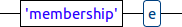
\includegraphics[scale=0.37]{./annex/images/membership.png}

\textbf{updates:} \hspace{5.4cm} \textbf{a:}\\
\vspace{0.2cm}
\hspace{1cm}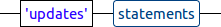
\includegraphics[scale=0.37]{./annex/images/updates.png} \hspace{4cm} 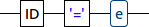
\includegraphics[scale=0.37]{./annex/images/a.png}

\end{figure}

\begin{figure}[!ht]
\textbf{prefixed:} \hspace{6.5cm} \textbf{e:}\\
\vspace{0.2cm}
\hspace{1cm}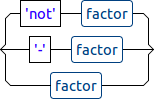
\includegraphics[scale=0.37]{./annex/images/prefixed.png} \hspace{5cm}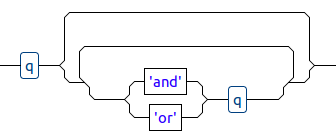
\includegraphics[scale=0.37]{./annex/images/e.png}

\textbf{q:}\\
\vspace{0.2cm}
\hspace{1cm}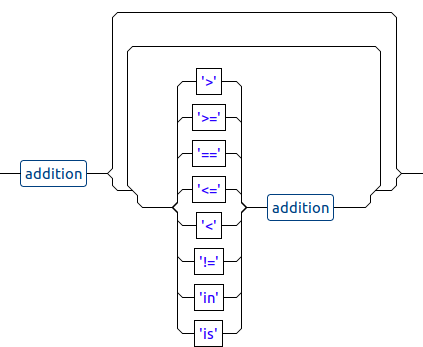
\includegraphics[scale=0.37]{./annex/images/q.png}

\textbf{addition:} \hspace{6cm} \textbf{term:}\\
\vspace{0.2cm}
\hspace{1cm}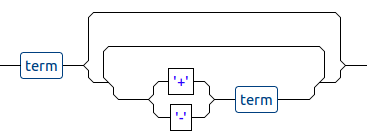
\includegraphics[scale=0.37]{./annex/images/addition.png} \hspace{3cm}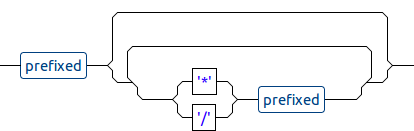
\includegraphics[scale=0.37]{./annex/images/term.png}

\textbf{factor:}\\
\vspace{0.2cm}
\hspace{1cm}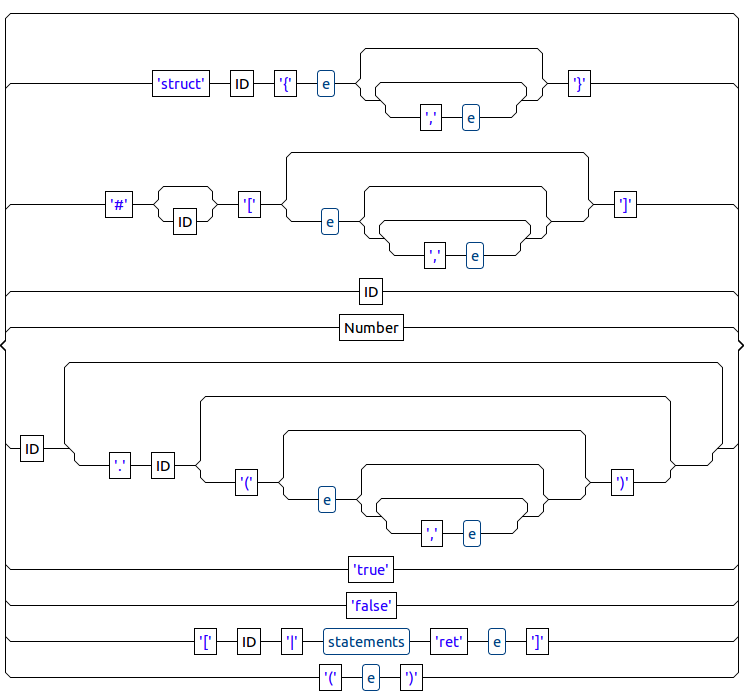
\includegraphics[scale=0.37]{./annex/images/factor.png}
\end{figure}